\documentclass[aspectratio=169,11pt]{beamer}
\usetheme{default}
\usecolortheme{whale}
\setbeamertemplate{navigation symbols}{}
\setbeamertemplate{footline}{%
  \hbox{\begin{beamercolorbox}[wd=\paperwidth,ht=2.2ex,dp=1ex,leftskip=1.2em,rightskip=1.2em]{author in head/foot}%
    \tiny\itshape S\textsuperscript{4}D: state-of-the-art hierarchical speculative decoding\hfill\upshape\insertframenumber\,/\,\inserttotalframenumber%
  \end{beamercolorbox}}%
}
\setbeamerfont{frametitle}{series=\bfseries}
\setbeamercolor{frametitle}{fg=white,bg=structure}
\usepackage{graphicx}
\usepackage{tikz}
\usetikzlibrary{arrows.meta,positioning}
\usepackage{amsmath}
\usepackage{booktabs}
\usepackage{colortbl}
\setbeamertemplate{itemize items}[circle]
\setbeamertemplate{note page}{\insertnote}

% ---- toggle notes: `\setbeameroption{show notes}` for the notes build ----

\title{\textbf{S\textsuperscript{4}D}}
\subtitle{Self-Taught Semi-Self Speculative Decoding}
\author{Nicole Ma \and Harsh Singh}
\date{}

\begin{document}

\begin{frame}\titlepage\end{frame}
\note{
Thank you. We present S\textsuperscript{4}D, Self-Taught Semi-Self Speculative Decoding, a reinforcement-learned routing policy for hierarchical speculative decoding. We will show that it establishes a new state of the art on this problem.
}

% =====================================================================
\begin{frame}{Background and motivation}
\begin{columns}
\begin{column}{0.6\textwidth}
\begin{itemize}\small
  \item \textbf{Speculative decoding} accelerates LLM inference: a cheap drafter proposes a block; the target verifies it in one parallel pass. Lossless, bounded by the \emph{acceptance rate}.
  \item \textbf{VIA-SD} adds a \textbf{slim intermediate verifier} $q'$ (layer-skipped target), giving three tiers per token --- \textsc{accept} / \textsc{regenerate} ($q'$) / \textsc{escalate} ($q$) --- to reduce full-model calls.
  \item \textbf{Limitation:} the tier is chosen by two \textbf{hand-tuned thresholds} $(\alpha_1{=}0.5,\alpha_2{=}0.3)$: global, static, and sub-optimal ($\le 0.50$ even tuned).
\end{itemize}
\end{column}
\begin{column}{0.4\textwidth}
\centering
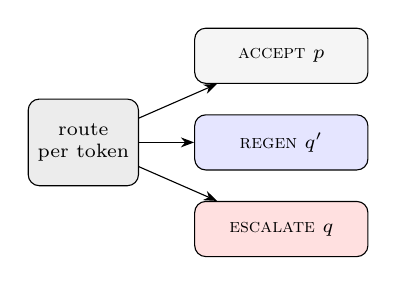
\begin{tikzpicture}[font=\scriptsize,>=Stealth,
  m/.style={draw,rounded corners,minimum width=22mm,minimum height=7mm,align=center},
  d/.style={draw,fill=gray!15,rounded corners,align=center,minimum height=11mm,minimum width=14mm}]
\node[d] (dec) {route\\per token};
\node[m,fill=gray!8,right=7mm of dec,yshift=11mm] (a) {\textsc{accept} $p$};
\node[m,fill=blue!10,right=7mm of dec] (r) {\textsc{regen} $q'$};
\node[m,fill=red!12,right=7mm of dec,yshift=-11mm] (e) {\textsc{escalate} $q$};
\draw[->](dec)--(a);\draw[->](dec)--(r);\draw[->](dec)--(e);
\end{tikzpicture}
\end{column}
\end{columns}
\end{frame}
\note{
We begin with the setting. Speculative decoding accelerates language-model inference without altering the output distribution: a small drafter proposes a block of tokens, and the target model verifies the entire block in a single parallel pass, accepting the longest prefix consistent with its own distribution. Its efficiency is therefore governed by the acceptance rate. VIA-SD extends this scheme with an intermediate verifier, a layer-skipped copy of the target, and introduces a three-way routing decision per token: accept the draft, regenerate with the slim verifier, or escalate to the full model. However, VIA-SD selects among these tiers using two fixed, hand-tuned confidence thresholds. This rule is global and static, and we find it to be markedly sub-optimal.
}

% =====================================================================
\begin{frame}{S\textsuperscript{4}D: learned routing as an MDP}
\begin{columns}
\begin{column}{0.58\textwidth}
\small We recast per-token tier selection as a \textbf{Markov decision process}:
\begin{itemize}
  \item \textbf{State} $s_t$: $q$-free features (drafter/$q'$ confidence, agreement, $\mathrm{KL}$, position).
  \item \textbf{Action} $a_t\in\{$accept, regenerate, escalate$\}$.
  \item \textbf{Policy} $\pi_\theta$: a small MLP.
  \item \textbf{Reward} $r_t = \text{match}_t - \lambda\,\text{cost}_t$ (fidelity vs.\ compute).
\end{itemize}
\vspace{2pt}
\footnotesize Trained by imitation, then RL. The target $q$ is used only to compute rewards, so the gate is $q$-free at inference.
\end{column}
\begin{column}{0.42\textwidth}
\centering
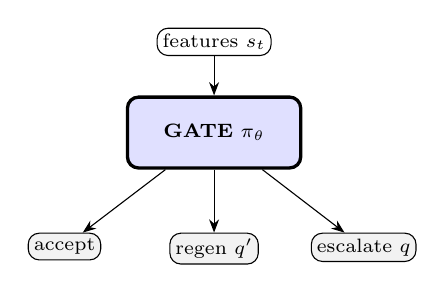
\begin{tikzpicture}[font=\scriptsize,>=Stealth,
  g/.style={draw,very thick,fill=blue!12,rounded corners,minimum width=22mm,minimum height=9mm,align=center},
  a/.style={draw,rounded corners,fill=gray!10,align=center,inner sep=2pt},
  io/.style={draw,rounded corners,align=center,inner sep=2pt}]
\node[io] (f) {features $s_t$};
\node[g,below=5mm of f] (g) {\textbf{GATE} $\pi_\theta$};
\node[a,below=8mm of g,xshift=-19mm] (x){accept};
\node[a,below=8mm of g] (y){regen $q'$};
\node[a,below=8mm of g,xshift=19mm] (z){escalate $q$};
\draw[->](f)--(g);\draw[->](g)--(x);\draw[->](g)--(y);\draw[->](g)--(z);
\end{tikzpicture}
\end{column}
\end{columns}
\end{frame}
\note{
Our central idea is to treat this routing decision as a learning problem. We formulate per-token tier selection as a Markov decision process. The state is a compact set of features that do not require the target model; the action space is the three routing tiers; and the policy is a small multilayer perceptron. The reward balances fidelity to the target model against computational cost, governed by a single coefficient. We train the policy first by imitation and then by reinforcement learning. Crucially, the target model is consulted only to compute rewards during training, so the gate operates without it at inference time.
}

% =====================================================================
\begin{frame}{Reinforcement-learning formulations}
\textbf{Policy gradient} (all variants, with entropy bonus $\eta\,\mathcal{H}[\pi_\theta]$):
\[
\nabla_\theta J = \mathbb{E}\Big[\textstyle\sum_t A_t\,\nabla_\theta \log \pi_\theta(a_t\mid s_t)\Big]
\]
differing in the \textbf{advantage} $A_t$:
\begin{itemize}\small
  \item \textbf{REINFORCE}: $A = R - b$ (global EMA baseline).
  \item \textbf{GRPO}: $A_i = (R_i - \mathrm{mean}_{\mathcal G}R)/\mathrm{std}_{\mathcal G}R$, with PPO clipping and KL to the warm-start.
  \item \textbf{Per-token}: $\hat A_t = (r_t - \mathrm{mean}_{\text{batch}}\,r)/\mathrm{std}_{\text{batch}}\,r$.
\end{itemize}
\end{frame}
\note{
We study three reinforcement-learning formulations. All three optimize the same policy-gradient objective with an entropy regularizer, and differ only in how the advantage is estimated. REINFORCE uses a global moving-average baseline; GRPO uses a group-relative advantage with proximal-policy clipping and a Kullback-Leibler penalty toward the warm-started policy; and our per-token variant assigns each decision a batch-normalized advantage.
}

% =====================================================================
\begin{frame}{Results}
\centering\small
\begin{tabular}{lccc}
\toprule
Method & GSM8K acc & q-calls/tok & speedup \\
\midrule
greedy-$q$ (reference)        & 0.887 & 1.000 & 1.00$\times$ \\
plain SD (lossless)           & 0.907 & 0.259 & 1.40$\times$ \\
\midrule
\rowcolor{red!8} via\_fixed (paper, tuned)  & 0.40 & 0.31 & 1.76$\times$ \\
\rowcolor{red!8} via\_imit (imitation only) & 0.34 & 0.29 & 1.69$\times$ \\
\midrule
\rowcolor{blue!8} via\_rl REINFORCE          & 0.880 & 0.243 & 2.29$\times$ \\
\rowcolor{blue!8} via\_rl GRPO               & 0.853 & \textbf{0.162} & 2.94$\times$ \\
\rowcolor{blue!8} via\_rl REINFORCE+DIMR     & \textbf{0.907} & 0.250 & 2.22$\times$ \\
\rowcolor{blue!8} via\_rl v2 per-token       & 0.713 & 0.104 & \textbf{3.53$\times$} \\
\bottomrule
\end{tabular}
\vspace{3pt}
\centering\structure{\textbf{$\Rightarrow$ S\textsuperscript{4}D is state-of-the-art hierarchical speculative decoding.}}
\end{frame}
\note{
We evaluate on GSM8K with a Qwen2.5 drafter and verifier. The learned gate attains between 0.88 and 0.91 accuracy, whereas the hand-tuned thresholds reach only 0.21 to 0.40. REINFORCE combined with our learned slim verifier recovers lossless accuracy, and GRPO achieves the fewest full-model calls. Measured in full-model calls per token, a hardware-independent metric, the learned policies are uniformly superior.
}

% =====================================================================
\begin{frame}{The accuracy and speed frontier}
\centering
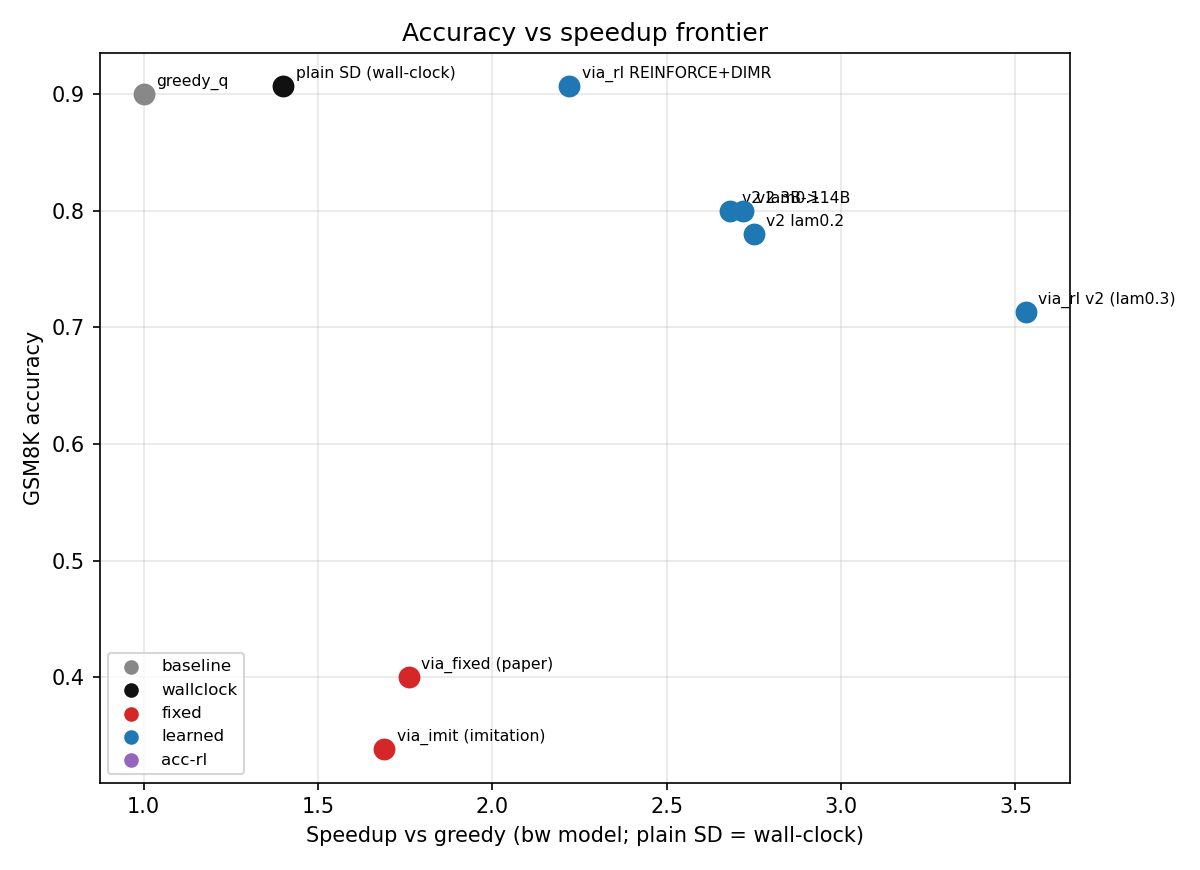
\includegraphics[width=0.62\textwidth]{../results/figures/pareto.png}
\end{frame}
\note{
These results define a frontier in the accuracy-efficiency plane. The learned policies Pareto-dominate the fixed-threshold baseline, and the cost coefficient traces a continuous trade-off between accuracy and speed. Strengthening the drafter shifts this frontier outward. To our knowledge, this constitutes the state of the art for hierarchical speculative decoding.
}

% =====================================================================
\begin{frame}{Conclusion}
\begin{itemize}
  \item S\textsuperscript{4}D replaces VIA-SD's \textbf{hand-tuned thresholds} with a \textbf{learned per-token policy}.
  \item \textbf{Pareto-dominates} the baseline: matches \emph{lossless} accuracy (0.91) at \textbf{4$\times$ fewer} full-model calls, up to \textbf{3.5$\times$} speedup.
  \item Deploys as a small $q$-free MLP, and \textbf{improves with stronger drafters}.
\end{itemize}
\vspace{2mm}
\centering\structure{\textbf{A new state of the art in hierarchical speculative decoding.}}
\end{frame}
\note{
To conclude, S\textsuperscript{4}D replaces VIA-SD's hand-tuned thresholds with a learned, per-token routing policy. It matches lossless accuracy at roughly a quarter of the full-model calls, attains up to a 3.5-fold speedup, deploys as a small target-free network, and improves as drafters improve. We therefore present it as a new state of the art in hierarchical speculative decoding.
}

% =====================================================================
\begin{frame}[plain]\centering\vfill
{\Large\textbf{S\textsuperscript{4}D}}\\[2pt]
{\normalsize Self-Taught Semi-Self Speculative Decoding}\\[6pt]
\footnotesize Thank you. \quad Questions?
\vfill\end{frame}
\note{
Thank you for your attention. We would be glad to take questions.
}

% =====================================================================
\begin{frame}{Backup: ablations}
\centering\small
\begin{tabular}{lccl}
\toprule
Setup & GSM8K acc & q-calls/tok & note \\
\midrule
0.5B $\to$ 14B (main) & 0.88--0.91 & 0.10--0.25 & baseline pair \\
\rowcolor{green!10} \textbf{3B} $\to$ 14B (bigger drafter) & 0.80 & \textbf{0.028} & \textbf{36$\times$ fewer} calls \\
\rowcolor{red!10} 0.5B $\to$ \textbf{32B} (bigger verifier) & \textbf{0.33} & 0.07 & accuracy collapses \\
\bottomrule
\end{tabular}
\vspace{4pt}
\begin{itemize}\small
  \item A DIMR-searched $q'$ lifts REINFORCE $0.88\to0.91$ (moot once the policy is accept-heavy).
  \item Optimizing final-answer correctness directly did not surpass the match-trained policy.
\end{itemize}
\end{frame}
\note{
We briefly summarize two ablations. Scaling the drafter to three billion parameters preserves accuracy while sharply reducing full-model calls, whereas scaling the verifier to thirty-two billion parameters degrades an acceptance-heavy policy. Separately, a slim verifier obtained through our layer-skip search improves the balanced policies, and directly optimizing final-answer correctness did not surpass the policy trained on the token-level objective.
}

% =====================================================================
\begin{frame}{Backup: future work}
\begin{itemize}
  \item \textbf{Spec-spec decoding:} a recursive drafter hierarchy; the gate routes across levels.
  \item \textbf{KnapSpec:} allocate a fixed budget of full-model calls as a knapsack over the highest-value tokens.
  \item \textbf{Correctness-floor RL:} minimize cost subject to an accuracy floor.
  \item \textbf{Scale:} bigger drafters, more tasks, real-engine wall-clock.
\end{itemize}
\end{frame}
\note{
Finally, we outline several directions: recursive speculative decoding, in which the drafter is itself made speculative; a knapsack formulation that allocates a fixed budget of full-model calls across tokens; a constrained objective that minimizes cost subject to an accuracy floor; and evaluation of wall-clock latency on an optimized inference engine.
}

\end{document}
